\documentclass{llncs}

\usepackage{graphicx}
\usepackage{placeins}

\begin{document}

\title{Artificial Neural Network Activation Function Optimization with Genetic Algorithms}

\author{Ivan Blagoev, Janeta Sevova, Kolyu Kolev}

\institute{Institute of Information and Communication Technologies \\
Bulgarian Academy of Sciences \\
acad. Georgi Bonchev Str, block 2, office 514, 1113 Sofia, Bulgaria \\
\email{i.blagoev@iit.bas.bg} \\
\texttt{http://www.iict.bas.bg/}}

%----------------------------------------------------------------------------------------
%   Title
%----------------------------------------------------------------------------------------

\maketitle

%----------------------------------------------------------------------------------------
%   Abstract
%----------------------------------------------------------------------------------------

\begin{abstract}

Artificial Neural Networks (ANNs) are widely used in the last few decades. They have application in many different areas as financial forecasting \cite{atanasova01,atanasova02,balabanov04,tomov01}, board and puzzle games \cite{balabanov01,balabanov03,keremedchiev01}, image processing, object classification, computer networks \cite{tashev01,tashev02} and many others. The most popular ANNs are represented as directed weighted graph in which signals are traveling from the input to the output. Each node (neuron) in these models have an activation function according which the node signal is emitted. The most popular activation functions are the sigmoid function and the hyperbolic tangent function \cite{zankinski01,balabanov02}. In this study evolutionary algorithms are employed in order to search for activation function alternatives. The function itself is represented as mathematical expression as the used in the genetic programming (GP).

\keywords{artificial neural networks, activation function, genetic algorithms, genetic programming}
\end{abstract}

%----------------------------------------------------------------------------------------
%   Paper
%----------------------------------------------------------------------------------------

\section{Introduction}

The main purpose of neuron's the activation function is to limit the strength of the emitted signal. The most common way of input signal collection is by sum of the signals multiplied by weight of the connections (Eq. \ref{equation01}).

\begin{equation}
\label{equation01}
y_{j} = \sum_{i=1}^{} x_{i}*w_{ij}
\end{equation}

Collecting the signals in such way is very dependant of the size in the previous layer of neurons. Also the values of the weights varietes a lot and the result of the Eq. \ref{equation01} can reach highg negative or positive values. Both problems are solved with normalization by usage of a neuron activation function. 

\begin{equation}
\label{equation02}
z_{j} = \frac{1}{1 + e^{-y_{j}}}
\end{equation}

\begin{equation}
\label{equation03}
z_{j} = \frac{e^{2y_{j}}-1}{e^{2y_{j}}+1}
\end{equation}

%\begin{figure}[h]
%  \centering
%  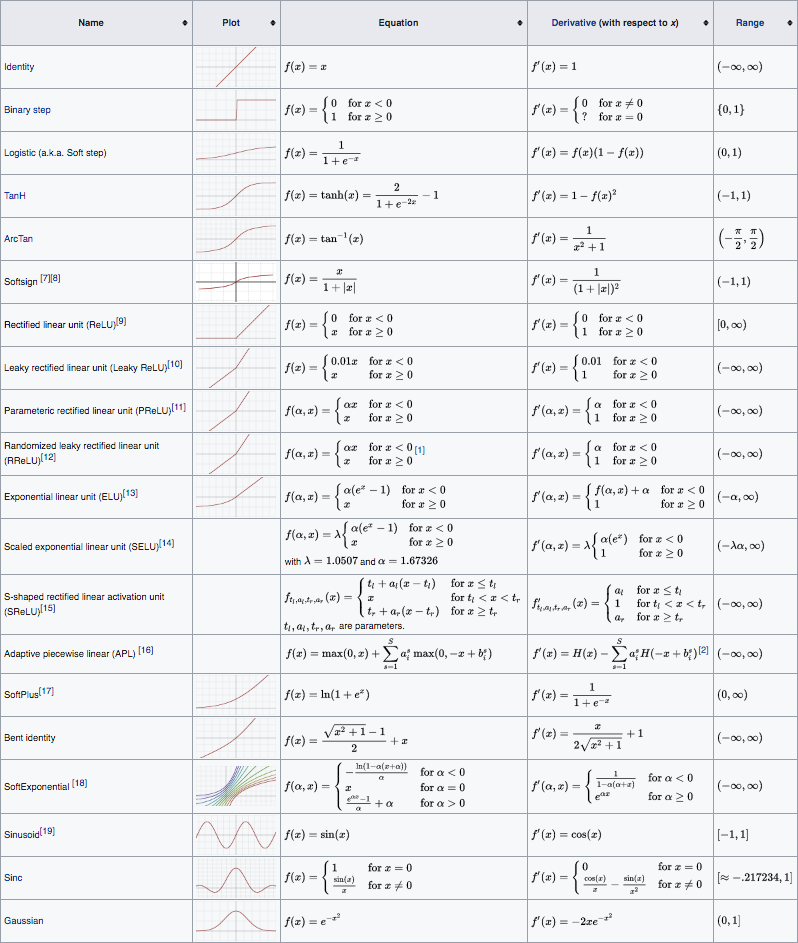
\includegraphics[height=0.5\pdfpageheight]{fig01}
%  \caption{List of most common activation functions \cite{wikipedia01}.}
%\label{fig01}
%\end{figure}
%\FloatBarrier

The most used functions are the sigmoid function (Eq. \ref{equation02}) and the hyperbolic tangent function (Eq. \ref{equation03}). List of less common used activation functions can be found at \cite{wikipedia01}.

\section{Activation Function Optimization}

The idea used in Radial Basis Function (RBF) ANNs for parameters optimization with Genetic Algorithms (GAs) \cite{awad01} can be extended to optimization of the activation function itself. The goal in such optimization is to find activation function expression which will reduce ANN training time without lost of ANN operation accuracy. Implementing ANN solutions with the Encog Machine Learning Framework allows usage of alternative activation functions \cite{zankinski01}. The expression of the alternative activation function can be easily represented with mXparser math expression library. The expression is stored and evaluated as text string. Activation function expressions as strings perfectly fit to the concept of the GP. Each string is represented as string chromosome and Apache Genetic Algorithms Framework is used for the chromosome evaluations. Initial GA population consists of valid randomly generated mathematical expressions. Single cut crossover is used and the random cut point is always on mathematical operator. As mutation random replacement with randomly selected mathematical operator is used. For fitness evaluate each expression is loaded in ANN neurons and total ANN efficiency is calculated. The total error for the neural network is used as fitness value. 

\section{Conclusions}

Investigations in the direction of searching for alternative activation functions can achieve interesting results, which may change the way in which ANNs are used. As further research it can be interesting the experiments with activation function to proceed in combination with permutational algorithms as it was described in \cite{zankinski02}.

%----------------------------------------------------------------------------------------
%   Acknowledgements
%----------------------------------------------------------------------------------------

\section*{Acknowledgements}

This work was supported by private funding of Velbazhd Software LLC.

%----------------------------------------------------------------------------------------
%   Bibliography
%----------------------------------------------------------------------------------------

\begin{thebibliography}{99}

\bibitem{atanasova01} Atanasova, T., Barova, M., Balabanov, T., \textit{Use of Neural Models for Analysis of Time Series in Big Data}, Publishing complex of "Vasil Levski" National Military University, ISSN 1314-1937, 193--198, 2016.

\bibitem{atanasova02} Atanasova, T., Atanasov, J., \textit{Use of Neural Models for Analysis of Time Series in Big Data}, Proceedings of the International Scientific Conference, UNITECH’16, Gabrovo, Bulgaria, ISSN 1313-230X,  207--212, 2016.

\bibitem{awad01} Awad, M., \textit{Optimization RBFNNs Parameters using Genetic Algorithms: Applied on Function Approximation}, International Journal of Computer Science and Security, vol. 4, issue 3, ISSN 1985-1553, 295--307, 2010.

\bibitem{balabanov01} Balabanov, T., Genova, K., \textit{Distributed System for Artificial Neural Networks Training Based on Mobile Devices}, Proceedings of the International Conference Automatics and Informatics, Sofia, Bulgaria, Federation of the Scientific Engineering Unions John Atanasoff Society of Automatics and Informatics, ISSN 1313-1850, 49--52, 2016.

\bibitem{balabanov02} Balabanov, T., Keremedchiev, D., Goranov, I., \textit{Web Distributed Computing For Evolutionary Training Of Artificial Neural Networks}, International Conference InfoTech, Varna - St. St. Constantine and Elena resort, Bulgaria, Publishing House of Technical University - Sofia, ISSN 1314-1023, 210--216, 2016.

\bibitem{balabanov03} Balabanov, T., Zankinski, I., Barova, M., \textit{Strategy for Individuals Distribution by Incident Nodes Participation in Star Topology of Distributed Evolutionary Algorithms}, Cybernetics and Information Technologies, Institute of Information and Communication Technologies - BAS, vol. 16, no. 1, ISSN 1311-9702, 80--88, 2016.

\bibitem{balabanov04} Balabanov, T., Zankinski, I., Dobrinkova, D., \textit{Time Series Prediction by Artificial Neural Networks and Differential Evolution in Distributed Environment}. Proceedings of the International Conference on Large-Scale Scientific Computing, Sozopol, Bulgaria, Lecture Notes in Computer Science, Springer, vol. 7116, no. 1, ISBN 978-3-642-29842-4, 198–205, 2011. 

\bibitem{keremedchiev01} Keremedchiev, D., Barova, M., Tomov, P., \textit{Mobile Application as Distributed Computing System for Artificial Neural Networks Training Used in Perfect Information Games}, Proceedings of the International Scientific Conference, UNITECH’16, Gabrovo, Bulgaria, ISSN 1313-230X, 389--393, 2016.

\bibitem{tashev01} Tashev, T., Marinov, M., Monov, V., Tasheva, R., \textit{Modeling of the MiMa-algorithm for crossbar switch by means of Generalized Nets}, Proceedings of the 2016 IEEE 8th International Conference on Intelligent Systems (IS), Sofia, Bulgaria, ISBN 978-1-5090-1354-8, 593--598, 2016.

\bibitem{tashev02} Tashev, T., Monov, V., \textit{Modeling of the hotspot load traffic for crossbar switch node by means of generalized nets}, Proceedings of the 6-th International IEEE Conference Intelligent Systems IS'12, Sofia, Bulgaria, vol. 2, 187--191, 2012.

\bibitem{tomov01} Tomov, P., Monov, V., \textit{Artificial Neural Networks and Differential Evolution Used for Time Series Forecasting in Distributed Environment}, Proceedings of the International Conference Automatics and Informatics, Sofia, Bulgaria, ISSN 1313-1850, 129--132, 2016.

\bibitem{zankinski01} Zankinski, I., Tomov, P., Balabanov, T., \textit{Alternative Activation Function Derivative in Artificial Neural Networks}, 25th Symposium with International Participation - Control of Energy, Industrial and Ecological Systems, Bankia, Bulgaria, John Atanasoff Union of Automation and Informatics, ISSN 1313-2237, 79--81, 2017.

\bibitem{zankinski02} Zankinski, I., Stoilov, T., \textit{Effect of the Neuron Permutation Problem on Training Artificial Neural Networks with Genetic Algorithms in Distributed Computing}, Proceedings of the 24th International Symposium Management of Energy, Industrial and Environmental Systems, ISSN 1313-2237, Bankya, Bulgaria, 53--55, 2016.

\bibitem{wikipedia01}  Wikipedia, \textit{Activation Function}, \\\texttt{https://en.wikipedia.org/wiki/Activation\_function}

\end{thebibliography}

\end{document}
